\subsection{Quadrant III. (Explicit Assurances, Informal Trust Treatment)}\label{sec:q3}
An AIA that can predict its performance on different tasks can provide assurances about competence, predictability, and the situational normality of a given task. Several authors have worked to improve this ability in visual classification \cite{Zhang2014-he,Gurau2016-hs,Churchill2015-ei,Kaipa2015-hy}. 
For example, to ensure that visual classifiers don't fail silently in novel scenarios, 
\citet{Zhang2014-he} learned models of errors on training images to predict errors on test images. 
\citet{Kaipa2015-hy} consider 3D visual classification of assembly line parts for robotic pick and place tasks, and develop statistical goodness-of-fit tests to estimate the likelihood that robots can use their sensors to find parts matching desired ones. %To accomplish this they apply the `Iterative Closest Point' (ICP) method, to match a point cloud measurement of the part with a ground-truth 3D model of the part. 
Each of these approaches enables the AIA to quantify its capability and present appropriate assurances to users, though without any formal considerations of user trust. 

%%The second paragraph that was here belongs entirely with self-confidence in previous section. I removed the text and shifted the references to Q2. These were explicitly papers about self-confidence, so I'm not sure why they were included here. 

Other assurances for machine learning algorithms are inspired by the well-known trade-off between accuracy and interpretability, whereby improving the accuracy of a learner generally reduces its interpretability. \citet{Ruping2006-xj} asks how classification results and the accuracy-interpretability trade-off can be made more transparent to those who design and use classifiers, by investigating the combined use of simpler global models and more complex local models that are built around learning results (\citet{Otte2013-oo} and \citet{Ribeiro2016-uc} implement similar ideas as well). 
Figure \ref{fig:ruping} illustrates this idea on a simple example: the left (global) model can be used as a large scale interpretable model of the learner's decision-making, while the more complex local model (shown on the right) can be used when more precise understanding of a specific decision made by the learner is required. 
%%While his focus was on classification, the methods could also be useful in regression as well.
\citet{Van_Belle2013-ph} suggested three ways to ascertain the level of interpretability and potential utility of learned models (compare to categories proposed by \citet{Lipton2016-ug}): 1) Map them to domain knowledge; 2) Ensure safe operation across the full operational range of model inputs; and 3) Assess whether important non-linear effects are accurately accounted for. 
This work identifies certain strengths and weaknesses of different techniques, but ultimately concludes that no method is clearly best in all situations. 
Along similar lines, \citet{Huysmans2011-th} compared decision trees, decision tables, propositional if-then rules, and oblique rule sets to understand which set of methods is `most interpretable'. 
It was experimentally determined that decision trees and tables tend to be easier to interpret, but it is noted that each method could perform better than others in different situations. 
While this gives some indication about how to choose classifiers for interpretability, \citeauthor{Park2016-ld} %, who investigated and proposed methods for making interpretable rules in decision trees, 
points out that \emph{real} interpretability in complex tasks still requires expert knowledge to make sense of complicated features. 
%For instance, \citet{Jovanovic2016-gw} use `Tree-Lasso' logistic regression with domain knowledge, i.e. medical diagnostic codes, to group similar conditions, and then use `Tree-Lasso' regression again on that information to develop a sparser model. 
%\citet{Zycinski2012-jj} also use domain knowledge to structure a data matrix before feature selection and classification. 
%%%%%%%%%%%%%%%%%%%%%%%%%
\begin{figure}[htbp]
    \centering
    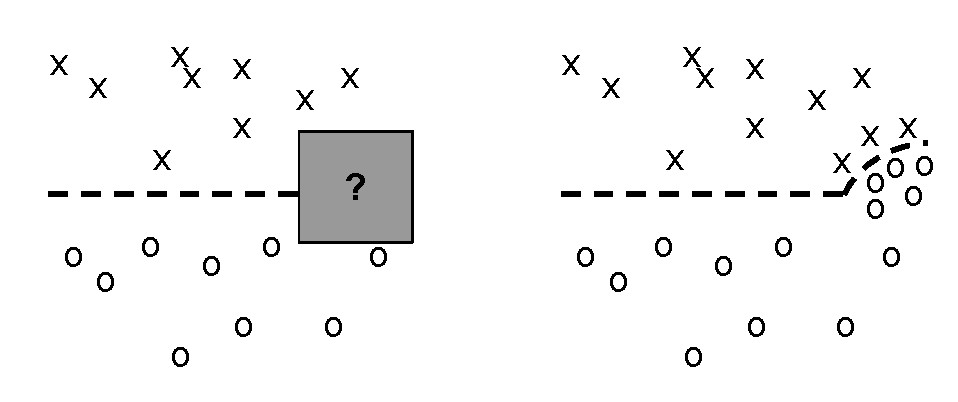
\includegraphics[width=0.65\textwidth]{Figures/global_local}
    \caption{Example of simple global interpretable learning model on the left, and on the right a more complex locally interpretable learning model that can be used when more detail is necessary.}
    \label{fig:ruping}
\end{figure}
%%%%%%%%%%%%%%%%%%%%%%%%%

\citet{Faghmous2014-og} argues that interpretable models are needed in data science when studying scientific phenomena such as environmental effects. They propose using `theory guided data science' (TGDS) to provide theoretically interpretable structures to data science problems. As one example of TGDS, \citet{Morrison2016-fz} address the situation where an imperfect analytical model is available for chemical reaction kinetics: the theoretical reaction equations are well known, but a `stochastic operator' is added on top of this to account for uncertainties and modeling errors. 
Several other research efforts have also aimed to make models more interpretable for a variety of learning applications, e.g. collaborative filtering using restricted Boltzmann machines \citet{Abdollahi2016-vn}, boosting using `weight of evidence' \citet{Ridgeway1998-lv}, and neural networks to exploit known `common sense' relationships between signals in different layers \citet{Choi2016-by}, just to name a few examples within this highly active research area. 
%There has been numerous other research efforts towards making models more interpretable. Generally the methods presented compete with (or excede) their state-of-the-art, less interpretable, counterparts. 
%\citet{Abdollahi2016-vn} investigate making collaborative filtering models more interpretable by using a conditional restricted Boltzmann machine (RBM). \citet{Ridgeway1998-lv} use `weight of evidence' (WoE) as a boosting method that is more amenable to interpretation, and show that WoE is on par with AdaBoost. \citet{Choi2016-by} construct a recursive attention neural network to remove recurrence on the hidden state vector, and instead add recurrence on the visits of patients to doctors, as well as on different diagnoses during those visits. In this way the model is able to predict possible diagnoses in time, and a visualization can be that that indicates the critical visits and diagnoses that lead to that prediction.  

One of the simplest approaches to helping users understand AIAs is to display the raw data being used, and rely on the user's own processing power to draw conclusions. In most real applications, however, there are too many individual variables for a human to attend to. Beyond that, users may have to be highly trained to interpret the results. In such situations, dimensionality reduction (DR) and visualization tools can be used to help make a model or data easier to understand. \citet{Venna2007-yj} discusses DR for ML and reviews many linear and non-linear projection methods. \citet{Vellido2012-nm} also discusses the importance of DR for making ML models interpretable. As one example, \citet{Chipman2005-om} applied this idea by constraining principle component analysis (PCA) in an attempt to make the resulting linear combinations of variables be more interpretable (more homogeneous, or more sparse).

%%\nisarcomm{need to massively compress the remaining 5 paragraphs -- WAAY too much detail...though some stuff for Lacave and Diez is very useful to port over to MURI and SAS proposal to highlight key differences from existing other programs/approaches...though we should spend more time on metacog state of art, which is more directly relevant...}
In some cases it is desirable to maintain a complex, less interpretable model and then apply `first principles' to explain the results to the user. \citet{Lacave2002-cu} address this from the perspective of explaining probabilistic inference in Bayesian networks -- specifically, \emph{how} and \emph{why} a Bayesian network reaches a conclusion given some imputed evidence. 
They present three properties of explanation: 1) content (what to explain), 2) communication (how to explain), and 3) adaptation (how to adapt based on who the user is). %%It is not possible to cover all of the ideas that they present in their paper, but they are key to the idea of designing assurances. 
Several key points for designing assurances arise from considering the differences between explaining evidence (i.e. data), the model (i.e. the Bayesian network itself), or the reasoning (i.e. the inference process). 
%These are three key considerations in making assurances. 
Also important is whether an explanation is meant to be descriptive or aimed at ensuring comprehension, as well as whether explanations need to be on a macro or micro scale relative for parts of the Bayesian network (similar to globally/locally interpretable learned models \citeauthor{Ruping2006-xj}). 
The authors also consider whether explanations should occur by two-way interaction between system and user, by natural language interaction, or by probabilities. Finally, considering adaptation, another key point for designing assurances in general applications and contexts is that not all users will require (or desire) the same kinds of assurances. This paper points out many challenges and considerations in designing assurances for probabilistic algorithms, and illustrates that (as with the `No free lunch' theorem) there is no single `best' assurance that will address every possible situation. 
Other discussion regarding how probabilistic and statistical explanations can be presented is found in \cite{Rouse1986-dz,Wallace2001-fm,Kuhn1997-qc,Lomas2012-ie,Swartout1983-ko}; 
as mentioned earlier, works such as \cite{Kuhn1997-qc} highlight the importance of framing effects and other cognitive biases in generating these kinds of explanations. 

Models and logic are not trustworthy by themselves; they may be flawed to begin with, or become invalid when certain assumptions or specifications are violated. Thus, there is also great interest in providing assurances that the models and assumptions underlying different AIA processes are in fact sound. \citet{Laskey1991-mf} -- with the intention of communicating model validity to users of `probability-based decision aids' -- notes that it is infeasible to perform a decision-theoretic calculation to determine if model revision is necessary. 
She then presents a class of theoretically justified model revision indicators which are based on the idea of constructing a computationally simple alternate model and then initiating model revision if the likelihood ratio of alternate model becomes too large (see also \citet{Zagorecki2015-qy,Habbema1976-xd} --these ideas also provide a potential basis for the `model validity' machine self-confidence factor described earlier in Quadrant II).

In the context of a practical self-driving car application, \citet{Ghosh2016-dl} presents a framework called Trusted Machine Learning (TML) for making ML models fit pre-determined `trustworthiness' constraints. 
Unlike most other kinds of assurances considered so far, these constraints are handed down by a certification authority as requirements to the ML system designer, and are not meant to be exposed to/determined by users. However, in principle, such hard assurances could be exposed to users in certain contexts. 
The key idea is to utilize tools from formal methods to provide theoretical proof of the functionality of the system. Note that, in the formal methods literature, such proofs and their supporting evidence are what are referred to as `assurances'; we earlier denoted these as `hard assurances', in contrast to the other kinds of `soft assurances' considered here. \nisarcomm{early on, we should make the distinction between `hard assurance's of the formal methods variety, and our variety of `soft assurances'}). 
\citet{Ghosh2016-dl}  present `model repair' and `data repair' strategies that can be used when the current model doesn't match the observed data, at which point the model and data can be repaired, and control actions can be replanned in order to conform with the formal method specifications. One challenge is how the `trustable' constraints should be identified, as this places a strong burden on the certifying authorities and system designer to foresee all possible failures. %, which is a strong assumption.

Another possible way to assure a human user of the trustworthiness of ML is to involve the human in the actual learning process. 
In theory, this provides an indirect way for users to build trust in the learning process by better understanding the `machine's perspective' (i.e. getting a sense for what it knows and doesn't know) and enabling mutual `calibration' of human-machine reasoning (rather than allowing users to simply attribute human understanding and learning processes onto the machine). 
For instance, \citet{Freitas2006-qo} compared two approaches to discovering `interesting' knowledge from large data sets, based on the idea that human users require assistance from complex systems in order to find useful patterns and other interesting insights. 
He mentions `user-driven' methods that involve a user suggesting interesting templates or providing general impressions in the form of IF-THEN rules. 
These are then compared to other `data-driven' methods, using other research to suggest that data-driven approaches are not very effective in practice. 
%%This is a cautionary tale that many times engineering methods to assist humans are not as effective as we would like to believe. 
However, user-driven approaches may not fair any better when compared over many users, as each user will likely have different preferences. 
Other scaled up user-driven approaches, e.g. based on crowd-sourcing \citet{Chang2017-kl}, can also achieve better accuracy for labeling tasks while also exploring new or ambiguous classes that can be ignored with traditional approaches (especially if training data sets are biased or very limited). 
%\citet{Chang2017-kl} also consider a similar, scaled up, `user-driven' approach called `Revolt' that crowd-sources the labeling of images. It is able to attain high accuracy labeling, while also exploring new or ambiguous classes that can be ignored with traditional approaches.

Finally, moving on from ML-oriented approaches, one can also consider approaches rooted in Validation and Verification (V\&V). V\&V typically refers to the use of formal methods to guarantee the performance of a system within in some set of specifications. However, not all practitioners are aware that V\&V provides ways to assure users. A prime example is given by \citet{Raman2013-mz}, who developed a way by which a user can provide natural language specifications to a robot and a `correct-by-construction' controller will be built if the specification is valid. Otherwise, the robot will provide an explanation about which specification(s) will cause failure. This approach is studied with the goal of implementing the system on a robot assistant in a hospital. Their method involves parsing natural language input (``Go to the kitchen''), and converting that into a linear temporal logic (LTL) task specification. This is then used to synthesize a robot controller if possible; otherwise, the `unrealizable' specifications are communicated back to the user. This approach is promising in that it presents a way to communicate that a specification cannot be met. But, it does not formally account for effects on user trust or TRBs in formulating explanations. The expression of assurances is also asymmetrically limited to cases where the robot cannot meet the specifications. 

\subsubsection{Summary}
    There are a few main approaches that researchers have used to create explicit assurances without formally considering trust models or effects:
    \begin{itemize}
        \item Making AIA capabilities more interpretable -- using techniques to simplify models, visualize data, explain reasoning and decision making, or to involve humans directly in the learning process. %is an attempt to create methods that are well-suited to convey assurances to human users. The output of these methods is the assurance, their interpretable form is well-suited to expressing that assurance.
        \item Predicting AIA performance -- %it is critical to predict performance in order for humans to understand how AIAs will behave in possible scenarios. By using methods that can predict performance, 
				designers can give AIAs the capability to explicitly communicate regarding competence, predictability, and situational normality to human users in different scenarios. 
        \item Ensuring capability of AIAs -- approaches such as model checking or formal V\&V allow the AIA to assess whether it is still functioning according to its design; this information can be quite useful in making explicit assurances for human users.
    \end{itemize}

The underlying hypothesis in this body of research is that the proposed methods \emph{should} affect the user's perception of the `competency' and `predictability' of the AIA, or the `situational normality' of the task being performed. However, none of this has been tested by user experimentation, e.g. that gathers and analyzes self-reported changes in trust. Similarly, there has been no formalization of how the effects that the proposed assurances have on TRBs might be quantified in different applications. In essence this work is only contains a small subset of important considerations for designing assurances, but includes several methods for assurance design. 
Indeed, the research in this quadrant is mainly focused on what AIA engineers and designers \emph{think} needs to be explained to or interpreted for users/stakeholders, or what assurance they \emph{think} users should have. 
These ideas definitely have merit, but need to be tested experimentally with users to determine whether they are in fact effective, to what extent they are effective, and whether there are more effective/efficient ways to achieve similar results. 
%Experimental testing of the effects of the proposed assurances on both self-reported trust, and TRBs remains open. 

